\documentclass[11pt]{article}
\usepackage[margin=1in]{geometry}
\usepackage[T1]{fontenc}
\usepackage[utf8]{inputenc}
\usepackage{lmodern}
\usepackage{hyperref}
\usepackage{booktabs}
\usepackage{enumitem}
\usepackage{amsmath}
\usepackage{pgfplots}
\pgfplotsset{compat=1.18}

\title{When Simplified Evaluators Misrank Policies: Protocol-Level Failure in Ledger-Constrained Market Learning}
\author{Anonymous Authors}
\date{}

\begin{document}
\maketitle

\begin{abstract}
Simplified evaluation can stop evaluating the policy that would actually be deployed. When settlement admissibility, welfare-sensitive outcomes, or protocol-level constraints are removed, the evaluator changes the object of comparison and can therefore distort policy ranking. We study that problem as \emph{evaluation protocol misspecification} in a seeded ledger-constrained market environment with explicit conservation/non-negativity/replay invariants, shared train / validation / held-out splits, and a compact retail-welfare decomposition. The central empirical result is protocol-level evaluation failure: on a matched calibrated four-policy slice, replacing the full protocol with \texttt{matching\_only} changes two of four ranks and yields Kendall $\tau=-0.20$; \texttt{no\_welfare\_reward} changes three of four ranks ($\tau=0.60$); and \texttt{no\_settlement} leaves the aggregate ranking unchanged ($\tau=1.0$) while weakening the admissibility boundary. Under the full protocol, controllers lie on a stable p99-latency--welfare frontier: methods that improve tail latency and fill throughput often widen surplus-transfer gap, while more balanced methods recover retail-sensitive outcomes only by paying latency cost. In the matched calibrated comparison, behavior cloning and IQL tie on the strongest held-out operating point, a transferred fitted-Q reference remains competitive but slower on tail latency, and stronger online value learning is checkpoint-sensitive enough that naive final-iterate reporting changes the apparent winner. These patterns persist under held-out regimes, welfare-weight perturbations, strategic-population shifts, stress sweeps, and a first-pass Binance spot calibration envelope. The resulting contribution is a reproducible ledger-aware evaluation protocol showing that simplified evaluators can change admissibility, rankings, and operating points even when the candidate policy set is fixed.
\end{abstract}

\section{Introduction}
Simplifying an evaluator can change the object being evaluated. If admissibility constraints, settlement semantics, or welfare-sensitive outcomes are removed from the loop, then controller comparisons are no longer performed on the same task, and empirical conclusions can change even before any new training is done.

This paper studies that problem as \emph{evaluation protocol misspecification}. The central question is not whether market infrastructure is complicated in the abstract. It is whether simplifying the evaluator changes feasibility, ranking, or operating point of the policies under comparison. Our empirical answer is yes. On a matched calibrated four-policy slice, \texttt{matching\_only} changes two of four ranks and yields Kendall $\tau=-0.20$; \texttt{no\_welfare\_reward} changes three of four ranks ($\tau=0.60$); and \texttt{no\_settlement} preserves ranking but weakens the admissibility boundary. These are not merely different summaries of the same result. They are protocol failures in which the evaluator itself changes what it means for one controller to outperform another.

We study the problem in a seeded ledger-constrained market environment that combines explicit conservation/non-negativity/replay checks, immediate and batched execution regimes, a shared adapter API, and a compact retail-welfare decomposition. We use this environment as a controlled instance of a broader ML question: when policies are compared under feasibility constraints and welfare-sensitive objectives, which protocol details are necessary to preserve the identity of the evaluated object? Under the full protocol, controllers lie on a stable latency--welfare frontier: aggressive latency optimization improves p99 and fill throughput but tends to widen surplus-transfer gap, while more balanced controllers recover retail-sensitive outcomes only by paying some latency cost. In the matched calibrated comparison, logged-data baselines outperform the online PPO-style baseline under shared train / validation / held-out rules, and stronger online value learning exposes checkpoint sensitivity as a first-class evaluation issue rather than an implementation footnote.

Counterfactual controls make the claim sharper. The first cross experiment holds the policy set fixed and swaps the evaluator: the full protocol is compared against \texttt{matching\_only} and \texttt{no\_settlement}. The second cross experiment keeps the ledger-aware evaluator but changes the training objective through \texttt{no\_welfare\_reward}. The point is therefore not that every infrastructure component is equally responsible for rank reversal. It is that simplified evaluation changes which conclusions survive, while settlement invariants define the correctness and admissibility boundary under which those conclusions should be trusted.

\paragraph{Why protocol matching matters.}
Existing market environments usually emphasize one of three things: historical-replay reinforcement-learning pipelines, multi-agent market simulation, or high-throughput order-book execution. This protocol study targets the gap between them. Mechanism effects, controller behavior, settlement semantics, and welfare-sensitive outcomes are often evaluated in separate layers even though production trading infrastructure couples them tightly. Real market replay also entangles mechanism effects with historical participant behavior and venue-specific structure. A seedable synthetic generator allows controlled stress testing of mechanism-controller interactions across arbitrage, retail, informed, and maker regimes that are difficult to isolate cleanly in historical data. The goal is therefore not just another market RL environment. It is to test whether simplifying the evaluation protocol changes what appears to be a good controller.

\begin{table}[t]
\centering
\footnotesize
\resizebox{\linewidth}{!}{%
\begin{tabular}{lccccc}
\toprule
Environment family & Synthetic/replay control & Mechanism variation & Settlement invariants & Learning API & Welfare summary \\
\midrule
FinRL-Meta-style replay suites \cite{liu2022finrlmeta} & replay-heavy & limited & no & yes & no \\
ABIDES-Gym-style simulators \cite{amrouni2021abidesgym} & yes & limited & no & yes & limited \\
JAX-LOB-style LOB simulators \cite{frey2023jaxlob} & mostly synthetic & LOB-focused & no & limited & no \\
This environment & yes, seedable & immediate/batch/adaptive & yes & yes & yes \\
\bottomrule
\end{tabular}
}
\caption{Positioning relative to existing market-environment families. The distinctive feature is a learning-facing evaluation protocol with explicit settlement invariants, mechanism variation, and retail-outcome summaries in the same loop.}
\end{table}

This paper makes four concrete contributions:
\begin{enumerate}[leftmargin=*]
  \item It defines \emph{protocol-level evaluation failure} in terms of feasibility failure, ranking failure, and operating-point failure, making explicit how evaluator simplification can change the admissibility set, the ranking of admissible policies, or the apparent Pareto surface.
  \item It introduces a reproducible ledger-aware evaluation protocol in which mechanism variation, learned controllers, deterministic settlement checks, and welfare-sensitive outcomes are evaluated under one shared train / validation / held-out design.
  \item It reports a matched calibrated comparison showing ranking reversal, frontier shift, and checkpoint sensitivity: behavior cloning and IQL dominate PPO under the matched protocol, while stronger online value learners reveal that final-iterate reporting can misstate the best available operating point.
  \item It strengthens the external-validity and robustness story with a stronger learner family, measurement-robustness checks, richer action-coverage diagnostics, and a first closed-loop calibration pass against a real Binance spot stylized-facts envelope.
\end{enumerate}

\section{Protocol-Level Evaluation Failure under Settlement Constraints}
We study a discrete-time environment in which a market state is advanced one simulator step at a time. At step $t$, the state is represented as
\[
s_t = (B_t, S_t, X_t, f_t),
\]
where $B_t$ and $S_t$ denote the buy and sell books, $X_t$ is the vector of account states, and $f_t$ is the latent synthetic fundamental used by the order-flow generator. A scenario additionally fixes a matching mode, a batch-window size, risk thresholds, and a population of agents.

The protocol study focuses on four concrete questions:
\begin{enumerate}[leftmargin=*]
  \item Do controller rankings change once settlement-aware and welfare-aware evaluation is used instead of matching-only summaries?
  \item How do immediate, speed-bump, adaptive, and frequent-batch-auction execution differ in latency, fill behavior, and retail-sensitive outcomes?
  \item Do offline/value-style and online learners exhibit different stability once checkpoint selection and held-out generalization are part of the protocol?
  \item Do settlement invariants and welfare-sensitive metrics remain reproducible and interpretable under heterogeneous agents, stress scenarios, and calibration?
\end{enumerate}

\subsection{Failure Definition}
Let $P_{\mathrm{full}}$ denote the full ledger-aware protocol and $P_{\mathrm{simp}}$ a simplified alternative such as matching-only evaluation or the no-welfare-reward control. Let $\Pi$ be a fixed candidate policy set. For a policy $\pi \in \Pi$, let
\[
A(\pi, P) \in \{0,1\}
\]
indicate admissibility under protocol $P$, where admissibility means zero conservation breaches and zero negative-balance violations. Let
\[
S(\pi, P) = z(\mathrm{fills/s}) - z(\mathrm{p99}) + z(\mathrm{retail\ surplus}) - z(\mathrm{retail\ adverse}) - z(\mathrm{surplus\ gap})
\]
denote the fixed evaluation score used for leaderboard-style comparisons among admissible policies under protocol $P$.

We say that $P_{\mathrm{simp}}$ induces \emph{protocol-level evaluation failure} on $\Pi$ relative to $P_{\mathrm{full}}$ if any of the following occur:
\begin{enumerate}[leftmargin=*]
  \item \textbf{Feasibility failure}: there exists $\pi \in \Pi$ such that $A(\pi, P_{\mathrm{simp}}) \neq A(\pi, P_{\mathrm{full}})$.
  \item \textbf{Ranking failure}: the ordering of admissible policies under $S(\cdot, P_{\mathrm{simp}})$ differs from the ordering under $S(\cdot, P_{\mathrm{full}})$, as witnessed by a top-1 reversal, a change in tied groups, or Kendall $\tau < 1$.
  \item \textbf{Operating-point failure}: even when admissibility and top-1 identity are preserved, the metric location of one or more policies or the non-dominated frontier shifts materially under a fixed metric set.
\end{enumerate}

This definition is evaluator-centric. \emph{Training objective misspecification} changes the optimization problem and therefore can change the learned policy itself. \emph{Evaluation protocol misspecification} changes the judgment rule applied to a fixed candidate policy set. The paper isolates the latter with cross-evaluator controls and uses \texttt{no\_welfare\_reward} as a bridge case showing that reward misspecification can amplify, but does not replace, evaluator misspecification. In the current artifact, the strongest evidence is for ranking failure and operating-point failure. \texttt{matching\_only} and \texttt{no\_welfare\_reward} alter controller ordering, whereas \texttt{no\_settlement} leaves the aggregate ordering unchanged and should therefore be interpreted more narrowly as isolating the correctness role of settlement rather than as evidence that settlement is irrelevant.

\section{Benchmark Environment}
\subsection{Core Components}
The environment couples seeded heterogeneous order flow, immediate/speed-bump/adaptive/batch execution, deterministic settlement application, and a metric layer that records systems, market-quality, and welfare-sensitive outcomes. Controllers interact with that environment through a common step-wise surface, \texttt{Reset()}, \texttt{Observe()}, \texttt{Step()}, and \texttt{Metrics()}, so heuristics, offline value learners, and online policy updates can be evaluated under one protocol.

The shared control bundle exposes five runtime channels: batch-window override for adaptive scenarios, risk-limit scaling, tie-break randomization, release-cadence control, and price-aggression bias \cite{brockman2016gym}. The goal is not to exhaust the control design space. It is to provide a small but nontrivial action surface on which evaluation protocol, admissibility, and welfare-sensitive outcomes can all matter at once.

\subsection{Determinism and Invariants}
Each scenario is seeded. Given the same scenario configuration and seed, the environment is expected to produce the same accepted order counts, fill counts, and benchmark metrics. The current protocol enforces three operational invariants:
\begin{enumerate}[leftmargin=*]
  \item \textbf{Conservation}: total cash and total inventory across accounts remain constant over time.
  \item \textbf{Non-negativity}: no account is allowed to end a fill application with negative cash or negative units.
  \item \textbf{Deterministic replay}: seeded runs produce stable outputs for the same configuration.
\end{enumerate}

\section{Agent Models}
The present environment includes four agent classes:
\begin{itemize}[leftmargin=*]
  \item \textbf{Market makers}: quote on both sides around the current fundamental with configurable width and intensity.
  \item \textbf{Latency arbitrageurs}: react to stale price information and attempt to exploit short-horizon dislocations.
  \item \textbf{Retail traders}: submit noisier buy or sell orders with wider dispersion around the current reference level.
  \item \textbf{Informed traders}: trade in the direction of the next-step fundamental when the generator exposes a directional signal.
\end{itemize}
These agents are intentionally simple. Their purpose is to generate heterogeneous but reproducible activity so that matching rules and controller choices can be compared under a repeatable workload. Richer strategic agents are a natural extension, but they are not required for the identification objective in its current form. To test whether the central result survives richer, state-dependent behavior, the artifact layer now also includes a strategic population with inventory-aware market makers, trend-reactive retail flow, signal-scaled informed traders, and dislocation-sensitive arbitrageurs.

\section{Tasks and Baselines}
The current environment suite contains fifteen scenarios:
\begin{enumerate}[leftmargin=*]
  \item \texttt{Immediate-Surrogate}
  \item \texttt{SpeedBump-50ms}
  \item \texttt{FBA-100ms}
  \item \texttt{FBA-250ms}
  \item \texttt{FBA-500ms}
  \item \texttt{Adaptive-100-250ms}
  \item \texttt{Adaptive-OrderFlow-100-250ms}
  \item \texttt{Adaptive-QueueLoad-100-250ms}
  \item \texttt{Policy-BurstAware-100-250ms}
  \item \texttt{Policy-LearnedLinUCB-100-250ms}
  \item \texttt{Policy-LearnedTinyMLP-100-250ms}
  \item \texttt{Policy-LearnedOfflineContextual-100-250ms}
  \item \texttt{Policy-LearnedFittedQ-100-250ms}
  \item \texttt{Policy-LearnedOnlineDQN-100-250ms}
  \item \texttt{FBA-250ms-Stress}
\end{enumerate}

The controller suite now contains a hand-written burst-aware controller, a contextual linear bandit, a gradient-trained TinyMLP policy, an offline contextual value controller, an offline fitted-Q controller, and an online DQN-style controller. The offline controllers are trained from logged trajectories generated by burst-aware, LinUCB, TinyMLP, offline contextual, and random behavior policies. The online controller is trained directly through adapter interaction over the same discrete action bundle. These controllers are included to isolate protocol effects across distinct learning styles rather than to claim a new learner family. Beyond the paper-facing base suite, the calibrated protocol also includes a behavior-cloning baseline on the shared logged-action split, a clipped PPO baseline, and an offline IQL-style baseline, while the artifact layer adds a prioritized Double-DQN style online controller. Taken together, the protocol suite now covers heuristic control, contextual bandits, supervised imitation, offline value learning, policy gradient, and stronger online value learning. The point is to test whether the protocol effect survives stronger learners, not to attribute the frontier to one weak baseline family.

\section{Metrics}
The environment reports five groups of signals:
\begin{itemize}[leftmargin=*]
  \item \textbf{Systems metrics}: orders per second, fills per second, and p50/p95/p99 latency.
  \item \textbf{Market-quality metrics}: average spread and average price impact.
  \item \textbf{Fairness-adjacent proxies}: queue-priority advantage, latency-arbitrage profit, and execution dispersion.
  \item \textbf{Primary welfare decomposition}: retail surplus per traded unit, retail adverse-selection rate, and surplus-transfer gap.
  \item \textbf{Secondary diagnostics}: arbitrageur surplus per traded unit and welfare dispersion.
  \item \textbf{Safety metrics}: negative-balance violations, conservation breaches, and risk rejections.
\end{itemize}
The welfare metrics should be interpreted as controlled outcome proxies inside the simulator environment rather than direct measurements of real-market welfare. Their purpose is to expose systematic tradeoffs between latency optimization and surplus transfer under a fixed synthetic fundamental, not to claim a universal welfare theorem for live markets. Their role in the protocol is nonetheless operational rather than decorative: across base and strategic population suites, surplus-transfer gap retains moderate positive correlation with queue advantage and price impact, and the welfare-gap ranking remains substantially stable across suites (Kendall $\tau = 0.6$). The measurement claim is therefore narrower than ``this is true welfare,'' but stronger than ``this is an arbitrary extra metric.''

\section{Experimental Protocol}
We separate exploratory sweeps from a paper-facing primary protocol. The primary protocol is the calibrated adaptive environment configuration with fixed train / validation / held-out splits, a shared observation schema, a shared six-action control bundle, and explicit checkpoint rules. The primary reported axes are p99 latency and surplus-transfer gap; fills per second and retail surplus are secondary interpretation metrics, and the artifact layer additionally exposes a standardized leaderboard score that combines these terms under one fixed formula. The paper's question is therefore not which learner wins after uncontrolled tuning. It is whether method conclusions survive once protocol, admissibility, and welfare-sensitive evaluation are fixed. All headline controller claims in the paper are tied to this fixed protocol rather than to exploratory curve maxima.

We report two result layers. The first is a single-seed reproducibility snapshot. The second is an eight-seed aggregate profile that is more appropriate for paper-facing discussion. The aggregate profile uses seeds
\[
[7, 11, 19, 23, 29, 31, 37, 41].
\]
The exploratory layer is used for multiseed mechanism profiles and learning-dynamics curves. In that layer, the learned fitted-Q controller uses a dedicated offline train/eval split: logged trajectories are collected on training seeds $[181, 191, 193, 197, 199, 211]$ from burst-aware, LinUCB, TinyMLP, offline contextual, and random behavior policies, then evaluated on held-out seeds $[223, 227, 229, 233]$. The online DQN-style controller uses replay-based Q-learning on training seeds $[307, 311, 313, 317, 331, 337]$, again with held-out evaluation on $[223, 227, 229, 233]$. These exploratory curves are useful for learning dynamics, but they are not the source of the paper-facing leaderboard claim.

The paper-facing primary protocol is the versioned calibrated adaptive environment configuration. It uses calibrated train seeds $[1103, 1109, 1117, 1123]$, validation seeds $[1129, 1151]$, and held-out seeds $[1153, 1163, 1171, 1181]$ over fixed validation and held-out regime families. To avoid selection bias, held-out regimes are never used for checkpoint choice. PPO selects the checkpoint with best validation score, IQL keeps the best validation iterate, behavior cloning reports a fixed final-epoch model under the same split, and the earlier fitted-Q policy is reported only as a transferred offline reference rather than as part of the matched train / validation protocol.

\begin{table}[t]
\centering
\footnotesize
\resizebox{\linewidth}{!}{%
\begin{tabular}{lllll}
\toprule
Track & Policies & Train data / seeds & Validation rule & Held-out role \\
\midrule
Exploratory base suite & \texttt{FittedQ}, \texttt{OnlineDQN} & offline logs on $[181,\dots,211]$ or online interaction on $[307,\dots,337]$ & none; final iterate used for curves & unseen stress regimes at $[223,\dots,233]$ for learning-dynamics analysis \\
Matched calibrated protocol & \texttt{behavior\_clone}, \texttt{ppo\_clip}, \texttt{iql} & calibrated train split on $[1103,1109,1117,1123]$ & fixed final epoch for BC; best validation checkpoint / iterate on $[1129,1151]$ for PPO/IQL & calibrated held-out report on $[1153,1163,1171,1181]$ only \\
Transferred calibrated reference & \texttt{fitted\_q} & offline logs from exploratory split & no recalibration; evaluated as-is & calibrated held-out comparison only \\
\bottomrule
\end{tabular}
}
\caption{Protocol summary. The key separation is between exploratory learning-dynamics artifacts and the matched calibrated comparison used for paper-facing method claims.}
\label{tab:protocolsummary}
\end{table}

All reported scenarios use the same simulator implementation and differ only in matching mode, batch-window size, seed, and population intensity. The current setup uses a discrete-time step duration of $10$ milliseconds.

\subsection{Learning Specification}
The learned controllers share one adapter interface. Observations contain seven scalars: a bias term, queue depth, buy/sell imbalance, spread, pending-order count, risk-rejection count, and normalized episode progress. The shared action bundle exposes six discrete control choices over batch-window target, risk-limit scale, tie-break mode, release cadence, and price-aggression bias.

The per-step reward shared by all learned controllers is
\begin{align*}
r_t ={}& 1.0 \cdot \Delta \text{fills}
- 0.25 \cdot \Delta \text{spread}
- 1.5 \cdot \Delta \text{impact}
- 12.0 \cdot |\Delta \text{queue}| \\
&- 0.005 \cdot \Delta \text{arb}
+ 18.0 \cdot \Delta \text{retail surplus}
- 10.0 \cdot \Delta \text{retail adverse}
- 2.0 \cdot \Delta \text{welfare dispersion} \\
&- 3.0 \cdot \max(\Delta \text{surplus gap}, 0)
- 0.5 \cdot \Delta \text{risk rejects}
- 10.0 \cdot \Delta \text{conservation breaches}.
\end{align*}

\begin{table}[t]
\centering
\footnotesize
\resizebox{\linewidth}{!}{%
\begin{tabular}{lllll}
\toprule
Controller & Function class & Training data / interaction & Main hyperparameters & Checkpoint rule \\
\midrule
\texttt{BehaviorClone} & TinyMLP classifier (hidden dim 10) & logged actions from burst-aware, LinUCB, TinyMLP, and offline contextual policies on calibrated train seeds & 12 supervised epochs, lr $0.022$, $L_2 = 10^{-4}$ & fixed final epoch; validation score reported but not used for early stopping \\
\texttt{FittedQ} & linear per-action values & offline trajectories from burst-aware, LinUCB, TinyMLP, offline contextual, and random policies on 6 exploratory train seeds & $\gamma=0.97$, 8 Bellman iterations, least-squares refit each round, target clamp $[-25,25]$ & snapshots $0..8$ on held-out regimes; iteration 8 reported \\
\texttt{PPOClip} & TinyMLP policy (hidden dim 12) & online interaction on calibrated train seeds & 80 episodes, clipped surrogate with $\epsilon=0.18$, 3 policy epochs per episode, lr $0.010$ & checkpoint every 10 episodes; best validation score reported \\
\texttt{IQL} & TinyMLP actor + linear critics & logged transitions from calibrated train seeds & 6 iterations, expectile $0.70$, beta $0.80$, weighted actor updates, lr $0.012$ & best validation iterate reported \\
\texttt{OnlineDQN} & TinyMLP Q-network (hidden dim 10) & online interaction on 6 exploratory train seeds with replay memory & $\gamma=0.97$, 160 episodes, $\epsilon: 0.25 \rightarrow 0.03$, replay cap 6000, updates after 48 samples, 4 Q-updates per step, lr 0.0035, $L_2 = 10^{-4}$, target refresh every 250 env steps & checkpoints every 20 episodes; episode 160 reported \\
\texttt{DoubleDQN} & TinyMLP Q-network (hidden dim 14) & online interaction on 6 exploratory train seeds with prioritized replay & $\gamma=0.97$, 200 episodes, $\epsilon: 0.20 \rightarrow 0.02$, replay cap 8000, updates after 64 samples, 6 Double-DQN updates per step, lr 0.0030, $L_2 = 10^{-4}$, Polyak target mix $\tau=0.08$ & checkpoints every 20 episodes evaluated on held-out regimes; curve reported separately \\
\bottomrule
\end{tabular}
}
\caption{Training specification for the matched calibrated baselines, the transferred fitted-Q reference, and the stronger Double-DQN artifact. These settings are intentionally controlled: the goal is to isolate protocol effects first, then test whether those effects survive stronger offline and online learners.}
\end{table}

The calibrated protocol layer extends that setup with a versioned train / validation / held-out split on the calibrated adaptive environment configuration. The calibrated-policy artifact reports five policies on validation and held-out regimes: \texttt{burst\_aware}, \texttt{behavior\_clone}, \texttt{fitted\_q}, \texttt{ppo\_clip}, and \texttt{iql}. Only three of them should be read as a matched protocol family: \texttt{behavior\_clone}, \texttt{ppo\_clip}, and \texttt{iql} share the same observation schema, discrete action bundle, calibrated train / validation / held-out split, and evaluation budget. \texttt{fitted\_q} remains useful, but it is a transferred offline reference trained under the earlier exploratory split rather than a member of the matched calibrated training protocol. This distinction matters because checkpoint rules and data splits are part of the protocol rather than incidental implementation details.

On the reference machine used for artifact generation, the unified hypercube run ($108$ cells, $4$ seeds per cell, $125$ steps per run) completes $54{,}000$ simulator steps in $19.42$ seconds, or about $2.78 \times 10^3$ steps per second; the runtime-profile artifact records the same measurement. Combining published per-cell throughput with episode duration yields an estimated wall-clock rate of $5.11 \times 10^4$ order events per second and $2.38 \times 10^4$ fills per second, which is sufficient for the lightweight offline and online learning experiments reported here.

\begin{figure}[t]
\centering
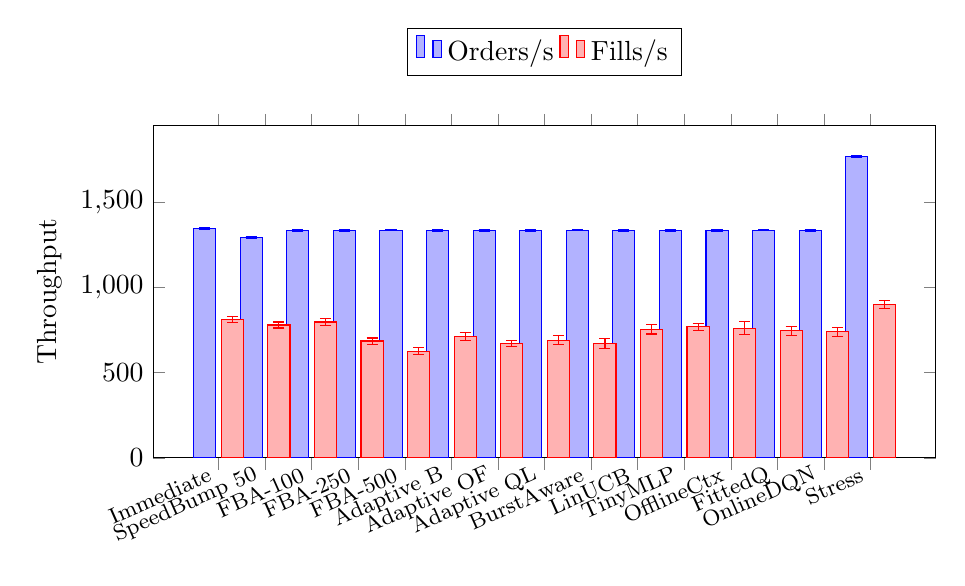
\begin{tikzpicture}
\begin{axis}[
    width=0.95\linewidth,
    height=5.8cm,
    ybar,
    bar width=8pt,
    ymin=0,
    symbolic x coords={Immediate,SpeedBump 50,FBA-100,FBA-250,FBA-500,Adaptive B,Adaptive OF,Adaptive QL,BurstAware,LinUCB,TinyMLP,OfflineCtx,FittedQ,OnlineDQN,Stress},
    xtick=data,
    xticklabel style={rotate=24,anchor=east,font=\footnotesize},
    ylabel={Throughput},
    legend style={at={(0.5,1.15)},anchor=south,legend columns=2},
    error bars/y dir=both,
    error bars/y explicit,
]
\addplot coordinates {(Immediate,1348.23) +- (0,3.99) (SpeedBump 50,1294.30) +- (0,3.84) (FBA-100,1337.09) +- (0,3.96) (FBA-250,1337.60) +- (0,3.88) (FBA-500,1338.82) +- (0,3.24) (Adaptive B,1337.60) +- (0,3.88) (Adaptive OF,1337.60) +- (0,3.88) (Adaptive QL,1337.60) +- (0,3.88) (BurstAware,1338.89) +- (0,2.97) (LinUCB,1337.60) +- (0,3.88) (TinyMLP,1337.60) +- (0,3.88) (OfflineCtx,1337.40) +- (0,3.91) (FittedQ,1337.70) +- (0,3.86) (OnlineDQN,1337.60) +- (0,3.88) (Stress,1769.25) +- (0,6.04)};
\addplot coordinates {(Immediate,813.13) +- (0,18.47) (SpeedBump 50,780.60) +- (0,17.73) (FBA-100,798.66) +- (0,21.71) (FBA-250,686.41) +- (0,17.80) (FBA-500,626.90) +- (0,19.72) (Adaptive B,714.29) +- (0,22.20) (Adaptive OF,671.43) +- (0,15.81) (Adaptive QL,691.57) +- (0,27.02) (BurstAware,670.83) +- (0,28.54) (LinUCB,755.65) +- (0,27.48) (TinyMLP,769.35) +- (0,20.85) (OfflineCtx,762.80) +- (0,36.22) (FittedQ,746.23) +- (0,27.90) (OnlineDQN,740.77) +- (0,26.35) (Stress,900.50) +- (0,23.67)};
\legend{Orders/s,Fills/s}
\end{axis}
\end{tikzpicture}
\caption{Aggregate throughput comparison with 95\% confidence-interval error bars.}
\end{figure}

\section{Results}
The results are organized around four layers: the latency--welfare frontier itself, learning dynamics, protocol effects, and robustness under calibration and stress. The main claim is not only that a latency--welfare conflict exists. It is that simplified evaluation protocols can hide or distort that conflict, while the full protocol exposes stable differences between controller families. Accordingly, Figure~\ref{fig:protocolranks}, Table~\ref{tab:checkpointprotocol}, and Figure~\ref{fig:paretofrontier} should be read as the primary result set, with learning curves and auxiliary leaderboards serving as supporting diagnostics.

\begin{figure}[t]
\centering
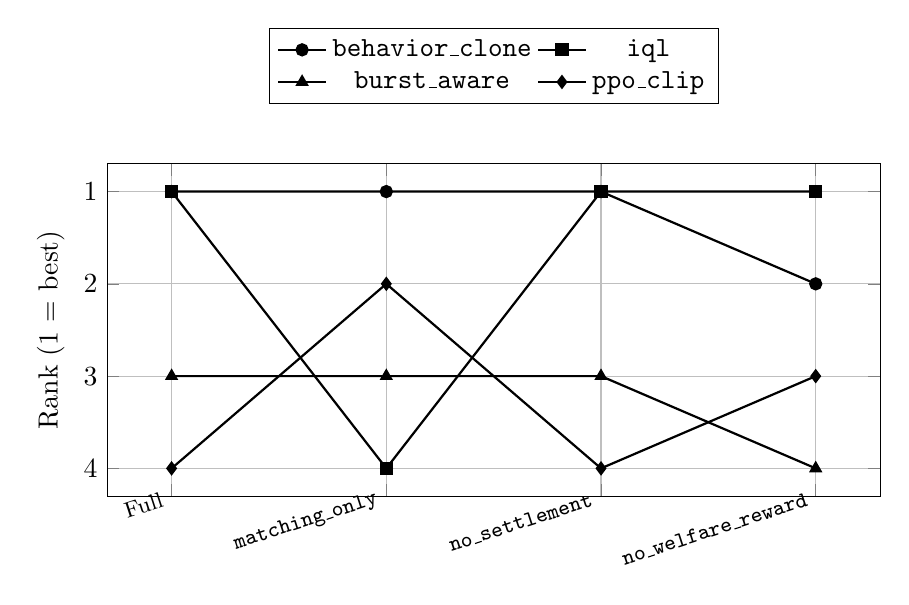
\begin{tikzpicture}
\begin{axis}[
    width=0.94\linewidth,
    height=5.8cm,
    xmin=0.7,
    xmax=4.3,
    ymin=0.7,
    ymax=4.3,
    y dir=reverse,
    xtick={1,2,3,4},
    xticklabels={Full,\texttt{matching\_only},\texttt{no\_settlement},\texttt{no\_welfare\_reward}},
    xticklabel style={rotate=18,anchor=east,font=\footnotesize},
    ylabel={Rank (1 = best)},
    ytick={1,2,3,4},
    grid=major,
    legend style={at={(0.5,1.18)},anchor=south,legend columns=2},
]
\addplot[mark=*, thick] coordinates {(1,1) (2,1) (3,1) (4,2)};
\addplot[mark=square*, thick] coordinates {(1,1) (2,4) (3,1) (4,1)};
\addplot[mark=triangle*, thick] coordinates {(1,3) (2,3) (3,3) (4,4)};
\addplot[mark=diamond*, thick] coordinates {(1,4) (2,2) (3,4) (4,3)};
\legend{\texttt{behavior\_clone},\texttt{iql},\texttt{burst\_aware},\texttt{ppo\_clip}}
\end{axis}
\end{tikzpicture}
\caption{Method rankings change under evaluation protocol. The full ledger-aware protocol and \texttt{no\_settlement} agree on the same ordering, while \texttt{matching\_only} and \texttt{no\_welfare\_reward} materially reorder the policies.}
\label{fig:protocolranks}
\end{figure}

Figure~\ref{fig:protocolranks} is the most direct statement of protocol-level ranking failure. On this fixed matched four-policy slice, the full protocol places \texttt{behavior\_clone} and \texttt{iql} jointly at the top, but the \texttt{matching\_only} simplification breaks that tie and promotes the imitation policy over the value-style one while also lifting \texttt{ppo\_clip} above \texttt{burst\_aware}. The causal interpretation is also sharper than in earlier drafts. \texttt{matching\_only} collapses the release-cadence and batch-window dimensions back to immediate execution, so policies are effectively judged on a narrower latency/fills view. \texttt{no\_welfare\_reward} leaves the infrastructure loop intact but removes welfare-sensitive optimization pressure, which is enough to improve the PPO-style controller without eliminating the frontier. \texttt{no\_settlement} keeps the same ranking because, in the current aggregate setup, the ordering is dominated by matching and reward design rather than by settlement application itself. The protocol question is therefore not cosmetic. Changing the evaluation loop changes what appears to be a good controller.
\subsection{Aggregate Summary}
\begin{table}[t]
\centering
\begin{tabular}{lrrrr}
\toprule
Scenario & Orders/s & Fills/s & p50 (ms) & p99 (ms) \\
\midrule
Immediate-Surrogate & 1348.2 & 813.1 & 10.0 & 10.0 \\
SpeedBump-50ms & 1294.3 & 780.6 & 60.0 & 60.0 \\
FBA-100ms & 1337.1 & 798.7 & 46.3 & 146.3 \\
FBA-250ms & 1337.6 & 686.4 & 97.5 & 452.5 \\
FBA-500ms & 1338.8 & 626.9 & 213.8 & 835.0 \\
Adaptive-100-250ms & 1337.6 & 714.3 & 81.3 & 360.0 \\
Policy-BurstAware & 1338.9 & 670.8 & 98.8 & 400.0 \\
Policy-LearnedLinUCB & 1337.6 & 755.7 & 48.8 & 155.0 \\
Policy-LearnedTinyMLP & 1337.6 & 769.3 & 62.5 & 221.3 \\
Policy-LearnedOfflineContextual & 1337.4 & 762.8 & 65.0 & 215.0 \\
Policy-LearnedFittedQ & 1337.7 & 746.2 & 46.3 & 145.0 \\
Policy-LearnedOnlineDQN & 1337.6 & 740.8 & 46.3 & 145.0 \\
FBA-250ms-Stress & 1769.3 & 900.5 & 97.5 & 373.8 \\
\bottomrule
\end{tabular}
\caption{Eight-seed aggregate summary. All runs report zero conservation breaches and zero negative-balance violations.}
\end{table}

\begin{table}[t]
\centering
\begin{tabular}{lrrrr}
\toprule
Scenario & Impact & Queue Adv. & Retail Surplus & Welfare Gap \\
\midrule
Immediate-Surrogate & 3.38 & 0.0742 & -0.3710 & 2.0430 \\
FBA-250ms & 5.36 & 0.0273 & -0.3493 & 0.8896 \\
Adaptive-100-250ms & 4.71 & 0.0375 & -0.1508 & 0.0278 \\
Policy-BurstAware & 5.31 & 0.0305 & -0.2258 & 0.7579 \\
Policy-LearnedLinUCB & 5.90 & 0.0513 & 0.0795 & 2.1694 \\
Policy-LearnedTinyMLP & 5.22 & 0.0336 & -0.3128 & 1.9719 \\
Policy-LearnedOfflineContextual & 4.94 & 0.0294 & -0.1090 & 1.3769 \\
Policy-LearnedFittedQ & 5.88 & 0.0451 & 0.0742 & 2.2036 \\
Policy-LearnedOnlineDQN & 5.92 & 0.0431 & 0.0662 & 2.2472 \\
FBA-250ms-Stress & 5.35 & 0.0269 & -0.1494 & 0.3805 \\
\bottomrule
\end{tabular}
\caption{Aggregate market-quality, welfare, and fairness-adjacent summary metrics.}
\end{table}

\begin{figure}[t]
\centering
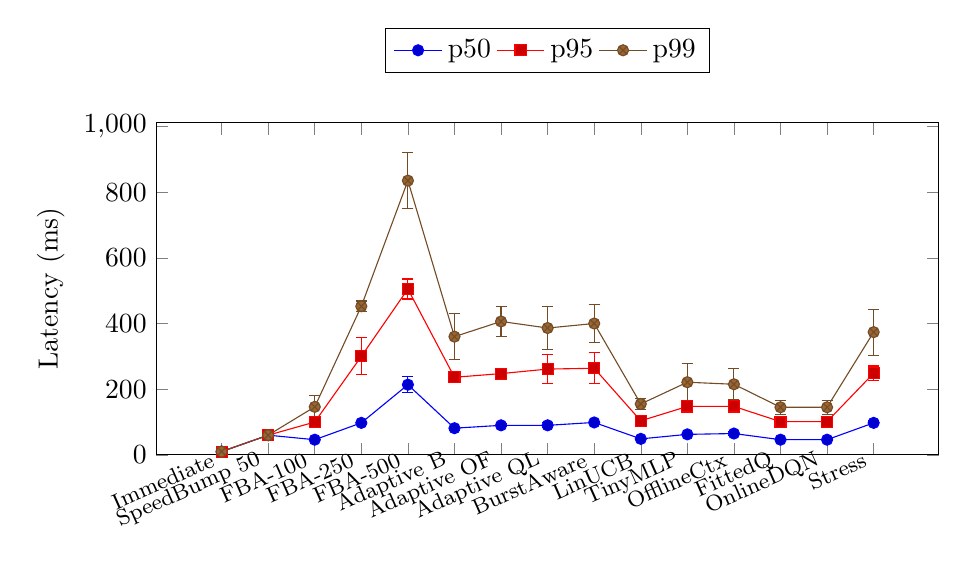
\begin{tikzpicture}
\begin{axis}[
    width=0.95\linewidth,
    height=5.8cm,
    ymin=0,
    symbolic x coords={Immediate,SpeedBump 50,FBA-100,FBA-250,FBA-500,Adaptive B,Adaptive OF,Adaptive QL,BurstAware,LinUCB,TinyMLP,OfflineCtx,FittedQ,OnlineDQN,Stress},
    xtick=data,
    xticklabel style={rotate=24,anchor=east,font=\footnotesize},
    ylabel={Latency (ms)},
    legend style={at={(0.5,1.15)},anchor=south,legend columns=3},
    mark=*,
    error bars/y dir=both,
    error bars/y explicit,
]
\addplot coordinates {(Immediate,10.0) +- (0,0.0) (SpeedBump 50,60.0) +- (0,0.0) (FBA-100,46.25) +- (0,3.35) (FBA-250,97.5) +- (0,4.58) (FBA-500,213.75) +- (0,24.48) (Adaptive B,81.25) +- (0,6.42) (Adaptive OF,90.0) +- (0,4.90) (Adaptive QL,90.0) +- (0,7.75) (BurstAware,98.75) +- (0,4.15) (LinUCB,48.75) +- (0,2.29) (TinyMLP,62.50) +- (0,3.00) (OfflineCtx,65.0) +- (0,6.00) (FittedQ,46.25) +- (0,3.35) (OnlineDQN,46.25) +- (0,3.35) (Stress,97.5) +- (0,5.75)};
\addplot coordinates {(Immediate,10.0) +- (0,0.0) (SpeedBump 50,60.0) +- (0,0.0) (FBA-100,100.0) +- (0,0.0) (FBA-250,300.0) +- (0,56.08) (FBA-500,505.0) +- (0,30.40) (Adaptive B,236.25) +- (0,10.92) (Adaptive OF,247.50) +- (0,6.71) (Adaptive QL,261.25) +- (0,44.83) (BurstAware,263.75) +- (0,47.63) (LinUCB,103.75) +- (0,4.82) (TinyMLP,147.50) +- (0,3.00) (OfflineCtx,147.50) +- (0,9.65) (FittedQ,101.25) +- (0,2.29) (OnlineDQN,101.25) +- (0,2.29) (Stress,248.75) +- (0,21.76)};
\addplot coordinates {(Immediate,10.0) +- (0,0.0) (SpeedBump 50,60.0) +- (0,0.0) (FBA-100,146.25) +- (0,35.83) (FBA-250,452.50) +- (0,16.16) (FBA-500,835.00) +- (0,84.37) (Adaptive B,360.0) +- (0,69.38) (Adaptive OF,406.25) +- (0,46.22) (Adaptive QL,386.25) +- (0,65.09) (BurstAware,400.0) +- (0,57.25) (LinUCB,155.0) +- (0,17.32) (TinyMLP,221.25) +- (0,57.40) (OfflineCtx,215.0) +- (0,47.25) (FittedQ,145.0) +- (0,21.36) (OnlineDQN,145.0) +- (0,21.36) (Stress,373.75) +- (0,70.24)};
\legend{p50,p95,p99}
\end{axis}
\end{tikzpicture}
\caption{Latency profiles with 95\% confidence intervals.}
\end{figure}

\begin{figure}[t]
\centering
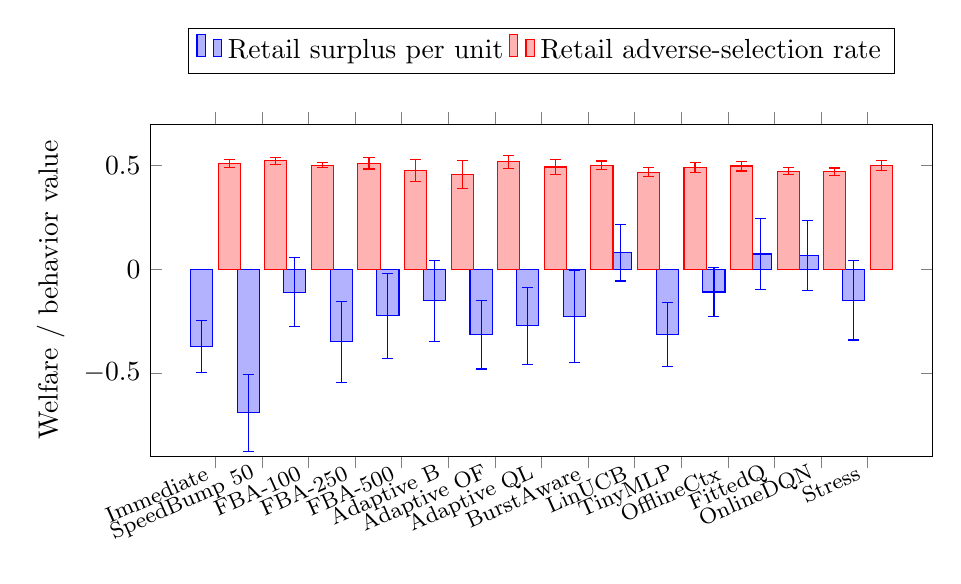
\begin{tikzpicture}
\begin{axis}[
    width=0.95\linewidth,
    height=5.8cm,
    ybar,
    bar width=8pt,
    ymin=-0.9,
    ymax=0.7,
    symbolic x coords={Immediate,SpeedBump 50,FBA-100,FBA-250,FBA-500,Adaptive B,Adaptive OF,Adaptive QL,BurstAware,LinUCB,TinyMLP,OfflineCtx,FittedQ,OnlineDQN,Stress},
    xtick=data,
    xticklabel style={rotate=24,anchor=east,font=\footnotesize},
    ylabel={Welfare / behavior value},
    legend style={at={(0.5,1.15)},anchor=south,legend columns=2},
    error bars/y dir=both,
    error bars/y explicit,
]
\addplot coordinates {(Immediate,-0.3710) +- (0,0.1264) (SpeedBump 50,-0.6903) +- (0,0.1854) (FBA-100,-0.1106) +- (0,0.1663) (FBA-250,-0.3493) +- (0,0.1951) (FBA-500,-0.2240) +- (0,0.2049) (Adaptive B,-0.1508) +- (0,0.1950) (Adaptive OF,-0.3139) +- (0,0.1656) (Adaptive QL,-0.2720) +- (0,0.1857) (BurstAware,-0.2258) +- (0,0.2212) (LinUCB,0.0795) +- (0,0.1353) (TinyMLP,-0.3128) +- (0,0.1535) (OfflineCtx,-0.1090) +- (0,0.1191) (FittedQ,0.0742) +- (0,0.1690) (OnlineDQN,0.0662) +- (0,0.1681) (Stress,-0.1494) +- (0,0.1905)};
\addplot coordinates {(Immediate,0.5109) +- (0,0.0183) (SpeedBump 50,0.5243) +- (0,0.0169) (FBA-100,0.5019) +- (0,0.0127) (FBA-250,0.5105) +- (0,0.0268) (FBA-500,0.4779) +- (0,0.0528) (Adaptive B,0.4562) +- (0,0.0682) (Adaptive OF,0.5178) +- (0,0.0315) (Adaptive QL,0.4935) +- (0,0.0369) (BurstAware,0.5019) +- (0,0.0203) (LinUCB,0.4690) +- (0,0.0231) (TinyMLP,0.4924) +- (0,0.0238) (OfflineCtx,0.4980) +- (0,0.0237) (FittedQ,0.4738) +- (0,0.0151) (OnlineDQN,0.4714) +- (0,0.0170) (Stress,0.4995) +- (0,0.0234)};
\legend{Retail surplus per unit,Retail adverse-selection rate}
\end{axis}
\end{tikzpicture}
\caption{Welfare and behavior signals with 95\% confidence intervals. Controllers that improve latency do not automatically improve retail outcomes.}
\end{figure}

\subsection{Observed Tradeoffs}
Four observations are currently the most informative.

First, immediate execution retains the lowest latency profile, but it also carries a high queue-advantage proxy and a large welfare gap. Under the current synthetic environment, low latency alone is not a good indicator of balanced market quality.

Second, the $50$ millisecond speed-bump baseline raises latency without reducing queue advantage. It preserves the immediate-style queue signal ($0.0742$) while worsening the welfare gap to $4.1034$. This makes it a useful negative control: latency rises, but batching-style fairness does not automatically follow.

Third, the fixed $250$ millisecond batch regime lowers queue advantage to $0.0273$ and compresses the welfare gap relative to immediate execution, but it gives up substantial tail latency. The balanced adaptive heuristic is the strongest fixed-logic mechanism on combined welfare terms: it keeps price impact low ($4.71$), reduces arbitrage-profit proxy to $522.00$, and nearly closes the welfare gap ($0.0278$).

Fourth, the controller comparison now exposes a clearer tradeoff than the earlier draft. \texttt{LinUCB} remains strong on tail latency and fill throughput, but it does so by widening both queue advantage and the surplus-transfer gap. \texttt{FittedQ} and \texttt{OnlineDQN} both produce the best in-distribution p99 tail ($145.0$ ms), giving explicit offline and online learning stories on top of the adapter API, but they still behave closer to \texttt{LinUCB} than to \texttt{OfflineContextual} on welfare transfer. \texttt{TinyMLP} improves fills further, but still leaves retail surplus negative and keeps arbitrage capture high. The offline contextual controller remains the strongest balanced learned baseline under the current protocol: compared with \texttt{LinUCB}, it gives up some tail latency but cuts price impact ($4.94$ versus $5.90$), lowers queue advantage ($0.0294$ versus $0.0513$), lowers arbitrage-profit proxy ($771.25$ versus $976.63$), and shrinks the welfare gap ($1.3769$ versus $2.1694$). This is already an evaluation effect: the methods that look strongest on p99 and fills are not the same methods that remain strongest once welfare-sensitive outcomes are treated as first-class metrics.

The stress scenario raises throughput to $1769.25$ orders per second and $900.50$ fills per second, but it also raises arbitrage capture to $2057.00$. Higher activity does not automatically imply better fairness or welfare outcomes.

Across all $15 \times 8 = 120$ aggregate runs, the environment reports zero negative-balance violations and zero conservation breaches.

\subsection{Held-Out Regime Generalization}
Held-out results use unseen seeds $[223,227,229,233]$ and four unseen regime combinations. The policy summary is shown in Table~\ref{tab:heldout}.

\begin{table}[t]
\centering
\begin{tabular}{lrrrr}
\toprule
Policy & Fills/s & p99 (ms) & Retail Surplus & Welfare Gap \\
\midrule
BurstAware & 834.08 & 376.88 & -0.4042 & 1.6286 \\
LinUCB & 978.52 & 171.25 & 0.1215 & 2.4466 \\
OfflineContextual & 961.61 & 275.62 & -0.0732 & 1.9535 \\
FittedQ & 946.78 & 159.38 & 0.1110 & 2.3158 \\
OnlineDQN & 986.61 & 172.50 & 0.0937 & 2.2189 \\
\bottomrule
\end{tabular}
\caption{Held-out policy summary over four unseen regimes.}
\label{tab:heldout}
\end{table}

The held-out picture is materially different from the in-distribution aggregate. \texttt{FittedQ} lowers both p99 and welfare gap relative to \texttt{LinUCB} in the high-arbitrage wide-maker, retail-burst, and composite-stress held-out regimes. In the informed-wide regime, it gives up some tail latency ($182.5$ versus $167.5$ ms) but still lowers welfare gap ($2.2994$ versus $2.3765$). \texttt{OfflineContextual} remains the most welfare-balanced learned baseline overall, but it is materially slower than both \texttt{LinUCB} and \texttt{FittedQ} on held-out tails. \texttt{OnlineDQN} sits between them: it improves held-out fills to $986.61$, keeps p99 at $172.50$ ms, and lowers the held-out welfare gap to $2.2189$, which is better than both \texttt{LinUCB} and \texttt{FittedQ} on this exploratory held-out aggregate. That result should be read narrowly. These exploratory policies are trained under different budgets and different data sources, so the section is evidence about learning dynamics and attainable operating points, not a clean protocol-level offline-versus-online comparison.

\subsection{Fitted-Q Learning Curve}
The fitted-Q controller is no longer just a point baseline. We also log its held-out behavior over Bellman-update iterations. The untrained snapshot begins at a welfare gap of $3.2117 \pm 0.5538$ and p99 latency of $341.25 \pm 22.97$ ms. After the first Bellman update, the held-out welfare gap falls to $2.0790 \pm 0.4767$ and p99 falls to $198.75 \pm 25.39$ ms. By iteration $8$, Bellman MSE declines from $45.1571$ to $6.5753$, held-out p99 reaches $155.62 \pm 12.84$ ms, and the welfare gap settles at $2.4226 \pm 0.5400$. The training story is therefore not monotone on every objective: later iterations improve Bellman error and tail latency, but they give back part of the earliest welfare improvement.

\begin{figure}[t]
\centering
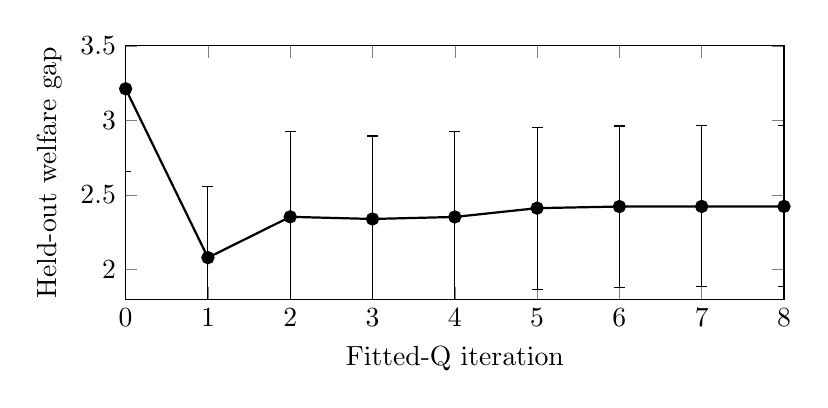
\begin{tikzpicture}
\begin{axis}[
    width=0.82\linewidth,
    height=4.8cm,
    ymin=1.8,
    ymax=3.5,
    xmin=0,
    xmax=8,
    xtick={0,1,2,3,4,5,6,7,8},
    ylabel={Held-out welfare gap},
    xlabel={Fitted-Q iteration},
    error bars/y dir=both,
    error bars/y explicit,
]
\addplot[mark=*, thick] coordinates {
    (0,3.2117) +- (0,0.5538)
    (1,2.0790) +- (0,0.4767)
    (2,2.3528) +- (0,0.5716)
    (3,2.3384) +- (0,0.5566)
    (4,2.3520) +- (0,0.5717)
    (5,2.4110) +- (0,0.5433)
    (6,2.4218) +- (0,0.5403)
    (7,2.4226) +- (0,0.5400)
    (8,2.4226) +- (0,0.5400)
};
\end{axis}
\end{tikzpicture}
\caption{Held-out fitted-Q learning curve. The first Bellman update captures most of the welfare-gap gain; later iterations continue to reduce Bellman error and tail latency but do not preserve that full early welfare improvement.}
\end{figure}

\subsection{Online DQN Learning Curve}
The online DQN-style controller adds a second, explicitly online training story. The untrained checkpoint begins at held-out p99 latency of $200.00 \pm 25.46$ ms and welfare gap of $1.5898 \pm 0.3869$. By episode $20$, held-out p99 falls to $155.62 \pm 12.84$ ms, while the welfare gap rises to $2.4226 \pm 0.5400$. Later checkpoints remain on the same plateau. The online controller therefore converges quickly toward a latency-favoring regime. Under the current reward structure, latency improvement is easier for the policy to exploit than retail-welfare preservation.

\subsection{Prioritized Double-DQN Extension}
The stronger online-RL artifact uses prioritized replay, Double-DQN targets, and Polyak target-network mixing. It does not change the paper's question, but it does add a materially stronger online-learning recipe than the plain DQN baseline. The untrained checkpoint starts at $875.55 \pm 145.75$ fills per second, $336.25 \pm 37.31$ ms p99 latency, and welfare gap $3.2567 \pm 0.6388$. By episode $80$, the controller reaches $1079.32 \pm 183.72$ fills per second with p99 latency $177.50 \pm 21.88$ ms and welfare gap $1.6813 \pm 0.4221$. By the final checkpoint at episode $200$, p99 falls further to $161.88 \pm 14.82$ ms, but the welfare gap widens back to $2.5926 \pm 0.5294$. The final iterate therefore improves p99 by only $15.62$ ms relative to episode $80$, while giving back $0.9113$ welfare-gap units and $145.64$ fills per second. The important result is not domination over the simpler DQN baseline. It is that a stronger online learner exposes a sharper checkpoint-selection tradeoff: later optimization can still pull the policy back toward a latency-favoring regime, so checkpoint selection must be treated as part of the evaluation protocol rather than as an afterthought.

\subsection{Reward Sensitivity}
To test whether the online-learning result depends on one hand-tuned reward vector, we retrain the online DQN controller under three deliberately separated reward profiles: the paper default, a latency-heavy profile, and a welfare-heavy profile. The final held-out operating point remains on the same plateau in all three cases. Default reward weights produce held-out p99 latency of $155.62 \pm 12.84$ ms and welfare gap $2.4226 \pm 0.5400$. The latency-heavy and welfare-heavy profiles produce the same held-out p99 and welfare-gap pair within the reported confidence intervals. The training reward scale changes materially, but the held-out controller behavior does not. For this protocol study, that is a useful robustness result: the latency-welfare tension is not only a consequence of one reward-weight vector. Under the current action bundle and held-out regimes, the online policy still converges toward the same latency-favoring operating region.

\begin{table}[t]
\centering
\begin{tabular}{lrrr}
\toprule
Profile & Mean train reward & Held-out p99 (ms) & Held-out welfare gap \\
\midrule
Default & 923.96 & 155.62 & 2.4226 \\
Latency-heavy & 1899.13 & 155.62 & 2.4226 \\
Welfare-heavy & -108.57 & 155.62 & 2.4226 \\
\bottomrule
\end{tabular}
\caption{Online DQN reward-sensitivity summary on held-out regimes. Large reward-weight perturbations change train reward scale but not the final held-out operating point.}
\end{table}

\subsection{First Closed-Loop Calibration Pass}
The study now includes a first closed-loop calibration pass against real public market data rather than only a synthetic generator. A stylized-facts envelope from an 8-symbol Binance spot slice is used to compare a baseline synthetic scenario against a tuned synthetic scenario. The calibration targets are explicit: spread, impact, and depth-shape statistics are the primary quantities being matched, while order-sign autocorrelation, inter-arrival timing, and volatility-clustering terms are checked but not yet tightly fit. This should therefore be read as a realism anchor with auditable error bounds rather than a claim of full market reconstruction.

The first-pass result is directionally strong even though it is not yet a final realism claim. The tuned generator moves mean spread from $326.41$ bps to $12.83$ bps, near the empirical upper envelope of $11.22$ bps, and moves the top impact bucket from $264.41$ bps to $8.47$ bps. It falls inside the empirical range on $7/13$ tracked summary metrics. The remaining misses are concentrated in order-sign autocorrelation, inter-arrival timing, one return-clustering term, and a subset of ask-side depth-shape statistics. In other words, the calibration materially improves the market-facing envelope, but it does not yet calibrate strategic adaptation, long-range dependence, or full equilibrium feedback.

More importantly for the paper's claim, the calibrated protocol profile keeps all calibrated scenarios at zero-breach while preserving the same qualitative latency--welfare tension as the base protocol:
\begin{itemize}[leftmargin=*]
  \item \texttt{Calibrated-Immediate-Surrogate}: $34.84 \pm 0.01$ orders/s, welfare gap $4.3321 \pm 0.1398$
  \item \texttt{Calibrated-FBA-2s}: $34.77 \pm 0.01$ orders/s, welfare gap $3.3927 \pm 0.1593$
  \item \texttt{Calibrated-Policy-LearnedFittedQ-1-3s}: $34.77 \pm 0.01$ orders/s, welfare gap $3.1301 \pm 0.1299$
\end{itemize}
The realism gap is therefore narrower than in earlier versions of the protocol, even though this remains a first-pass calibration rather than a high-fidelity market simulator. The central latency--welfare tension does not disappear once the synthetic generator is retuned toward a market-data envelope, which makes this calibration pass a useful external-validity anchor even while the paper's claim remains deliberately narrower than ``the simulator reproduces a live market.''

\subsection{Protocol Effects and Counterfactual Controls}
The raw market-data bundle is versioned with manifest hashes and per-file checksums in the artifact package. This does not turn simulator outputs into real-market results, but it does make the calibration input chain auditable and reproducible.

The calibrated-learning protocol now reports explicit train / validation / held-out splits rather than only a single tuned rerun. On held-out calibrated regimes, \texttt{burst\_aware} reaches $47.16 \pm 3.43$ fills per second with welfare gap $5.8322 \pm 0.1675$, \texttt{behavior\_clone} reaches $58.86 \pm 1.72$ fills per second with welfare gap $3.9602 \pm 0.2590$, \texttt{fitted\_q} reaches $56.86 \pm 1.89$ fills per second with welfare gap $3.9602 \pm 0.2672$, \texttt{ppo\_clip} reaches $40.54 \pm 1.85$ fills per second with welfare gap $6.6590 \pm 0.3586$, and \texttt{iql} reaches $58.86 \pm 1.72$ fills per second with welfare gap $3.9602 \pm 0.2590$. The strongest matched calibrated tradeoff therefore comes from logged-data baselines rather than from the PPO-style controller: \texttt{behavior\_clone} and \texttt{iql} tie on the best held-out point, while \texttt{fitted\_q} remains close but slower on p99 latency because it is transferred from the earlier offline split. A paired sign-flip comparison on the calibrated held-out regimes shows that \texttt{iql} improves both welfare gap and p99 latency relative to \texttt{ppo\_clip} with exact $p=3.1 \times 10^{-5}$ under the current protocol. The standardized calibrated leaderboard in \texttt{simulator\_policy\_leaderboard} therefore places \texttt{behavior\_clone} and \texttt{iql} jointly at the top, followed by \texttt{fitted\_q}, under one fixed score combining fills, p99, retail surplus, adverse selection, and surplus-transfer gap. Checkpoint sensitivity is therefore a main result rather than an appendix detail: once online learning is strong enough, the selection rule itself becomes part of the evaluation protocol because intermediate policies can dominate naive final iterates on the latency-welfare frontier.

One new diagnostic clarifies how this tied held-out point should be interpreted. The data-coverage artifact shows that the behavior-cloning split is not data-starved: it contains $7{,}696$ logged samples over $6{,}810$ rounded feature states and covers five of the six discrete actions, with mass split almost evenly between \texttt{balanced\_mid} ($49.29\%$) and \texttt{fast\_passive} ($49.14\%$). The IQL training set is broader still: $11{,}544$ transitions over $10{,}635$ rounded states with support on all six actions once random rollouts are added. Yet the policy-agreement artifact shows that \texttt{behavior\_clone} and \texttt{iql} choose the same action on $100\%$ of both validation and held-out reference states, and that action is \texttt{fast\_passive}. The present tie should therefore be read as a structural collapse of the current $7$-feature / $6$-action protocol to one operating point, not as evidence that another pass of the same training budget would separate the methods. This is why richer observation/action design is a next-step requirement rather than a cosmetic extension.

The counterfactual-control artifact provides the two cross experiments that separate evaluator misspecification from reward misspecification. First, holding the policy set fixed and swapping the evaluator shows protocol-level ranking failure directly. In \texttt{matching\_only}, p99 latency collapses to $1000$ ms but retail surplus stays negative and welfare gap remains large ($4.4725$ to $5.2132$ across published policies); more importantly, relative to the full control protocol, two of four ranks move and Kendall $\tau=-0.20$. In \texttt{no\_settlement}, the mechanism and welfare measurements remain unchanged while settlement application is removed, and the same policy ranking is preserved with Kendall $\tau=1.0$. Second, keeping the ledger-aware evaluator but changing the training objective through \texttt{no\_welfare\_reward} shows that objective misspecification can also distort comparison: the PPO-style controller improves to $54.49 \pm 4.34$ fills per second and $3312.50 \pm 227.12$ ms p99, but still leaves a substantial welfare gap at $3.3874 \pm 0.1272$; the protocol ranking changes again, with three of four policy ranks moving and Kendall $\tau=0.60$. These controls sharpen the claim. \texttt{matching\_only} is the main rank-reversal source, \texttt{no\_welfare\_reward} produces an even larger reordering, and \texttt{no\_settlement} should be read more narrowly as preserving the aggregate ordering while still defining correctness, admissibility, and the trust boundary under which a learned controller would be acceptable in infrastructure use.

\begin{table}[t]
\centering
\begin{tabular}{lccrr}
\toprule
Track & Selection rule & Selected iterate & Selected p99 (ms) & Selected gap \\
\midrule
\texttt{BehaviorClone} & fixed report rule & epoch 12 = final & 1500.00 & 3.9602 \\
\texttt{IQL} & best validation iterate & iter 6 = final & 1500.00 & 3.9602 \\
\texttt{PPOClip} & best validation checkpoint & episode 80 = final budget & 6000.00 & 6.6590 \\
\texttt{DoubleDQN} & dominant diagnostic checkpoint & episode 80 & 177.50 & 1.6813 \\
\texttt{DoubleDQN} & naive final iterate & episode 200 & 161.88 & 2.5926 \\
\bottomrule
\end{tabular}
\caption{Checkpoint sensitivity as a protocol choice. Under the matched calibrated protocol, reported iterates coincide with fixed final or best-validation rules. In the stronger exploratory Double-DQN run, the final iterate improves p99 but worsens welfare gap relative to the earlier dominant checkpoint.}
\label{tab:checkpointprotocol}
\end{table}

\subsection{Controller Pareto Frontier}
The multiseed controller frontier makes the same tradeoff visible on one surface. When minimizing p99 latency and surplus-transfer gap jointly, three points remain undominated: immediate execution, the balanced adaptive heuristic, and the offline contextual controller. Immediate execution is fastest but welfare-weak; the adaptive heuristic nearly closes the welfare gap but gives up substantial tail latency; offline contextual is the strongest balanced learned point. Figure~\ref{fig:paretofrontier} makes the operating-point story explicit: the relevant comparison is not a single scalar winner, but how protocols move policies along or away from the latency--welfare surface.

\begin{figure}[t]
\centering
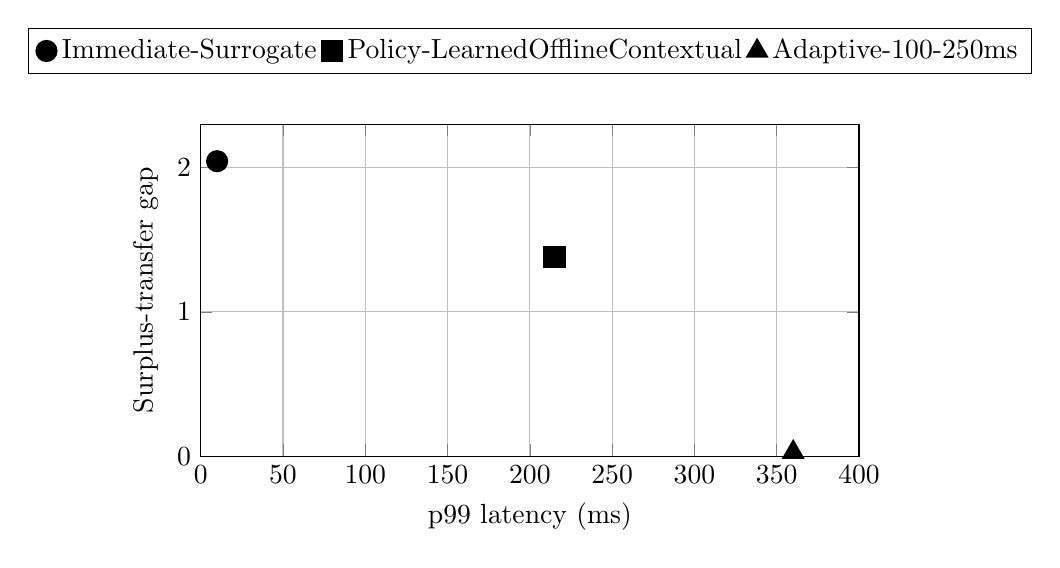
\begin{tikzpicture}
\begin{axis}[
    width=0.82\linewidth,
    height=5.8cm,
    xmin=0,
    xmax=400,
    ymin=0,
    ymax=2.3,
    xlabel={p99 latency (ms)},
    ylabel={Surplus-transfer gap},
    grid=major,
    legend style={at={(0.5,1.15)},anchor=south,legend columns=3},
]
\addplot[only marks, mark=*, mark size=3.6pt, thick] coordinates {(10,2.0430)};
\addplot[only marks, mark=square*, mark size=3.6pt, thick] coordinates {(215,1.3769)};
\addplot[only marks, mark=triangle*, mark size=4.0pt, thick] coordinates {(360,0.0278)};
\legend{Immediate-Surrogate,Policy-LearnedOfflineContextual,Adaptive-100-250ms}
\end{axis}
\end{tikzpicture}
\caption{p99 latency--welfare Pareto surface over the multiseed controller family. Immediate execution is fastest but welfare-weak; the adaptive heuristic minimizes welfare gap; offline contextual occupies the strongest balanced learned point.}
\label{fig:paretofrontier}
\end{figure}

\subsection{Metric Robustness and Stress Robustness}
Metric robustness is treated as a primary experiment rather than as appendix-only supporting evidence. Across base and strategic populations, surplus-transfer gap retains moderate positive correlation with queue advantage and price impact, while the welfare-gap ranking remains substantially stable across suites (Kendall $\tau=0.6$). This does not prove that the welfare proxy is unique or complete. It does show that the paper's main metric is structured, moderately stable, and not an arbitrary one-off summary. The appendix then retains mechanism ablations, agent/workload sweeps, and strategic-agent snapshots as stress tests showing that the main claim is not tied to one frozen population mix, one risk setting, or one single market-maker specification. Across those checks, the same directional pattern persists: relaxing risk raises throughput but also arbitrage capture, retail burst loads activity without neutralizing welfare transfer, and richer strategic agents preserve the same arbitrage-driven deterioration in retail outcome.

\begin{table}[t]
\centering
\begin{tabular}{lrr}
\toprule
Measurement check & Statistic & Value \\
\midrule
Gap vs queue advantage & Pearson correlation & 0.3305 \\
Gap vs price impact & Pearson correlation & 0.3417 \\
Base vs strategic ranking & Kendall $\tau$ on welfare gap & 0.6000 \\
\bottomrule
\end{tabular}
\caption{Compact measurement-robustness summary from the welfare artifact. The point is not that the proxy is perfect, but that it is structured and moderately stable rather than arbitrary.}
\end{table}

Finally, we expose a unified $4 \times 3 \times 3 \times 3$ hypercube over arbitrageur intensity $\{0,1,2,3\}$, retail intensity $\{1,2,3\}$, informed intensity $\{1,2,3\}$, and maker quote width $\{1,2,3\}$. Two raw cells still illustrate the environment directly. At $(\text{arb}=0,\text{retail}=1,\text{informed}=2,\text{maker}=1)$, the environment reports $1350.60$ orders per second, zero arbitrage-profit proxy, and a welfare gap of $0.2376$. At $(\text{arb}=3,\text{retail}=1,\text{informed}=2,\text{maker}=1)$, throughput rises to $1542.86$ and p99 falls to $362.50$ milliseconds, but arbitrage-profit proxy jumps to $1982.00$ and the welfare gap widens to $1.2839$.

\begin{table}[t]
\centering
\begin{tabular}{lrrrr}
\toprule
Factor & $\Delta$ Orders/s & $\Delta$ Retail Surplus & $\Delta$ Retail Adverse & $\Delta$ Welfare Gap \\
\midrule
Arbitrage $0 \rightarrow 3$ & 176.26 & -0.1804 & 0.0117 & 1.2099 \\
Retail $1 \rightarrow 3$ & 780.94 & 0.0772 & 0.0018 & 0.0781 \\
Informed $1 \rightarrow 3$ & 150.91 & -0.1986 & 0.0131 & 0.0876 \\
Maker width $1 \rightarrow 3$ & 0.00 & -0.1250 & 0.0085 & 0.2653 \\
\bottomrule
\end{tabular}
\caption{Compact high-low contrasts from the unified hypercube.}
\end{table}

This compact summary removes the need to interpret the hypercube only through slice families. Rather than reporting slice plots alone, the study summarizes the stress surface with response-surface fits and factor contrasts that expose the dominant drivers of welfare transfer. Arbitrage intensity consistently emerges as the dominant driver of welfare-gap expansion, retail intensity is mostly a throughput lever, and wider maker quotes worsen retail outcome without moving aggregate activity in this setup. Averaged over informed intensity and maker width, moving from $\text{arb}=0$ to $\text{arb}=3$ widens the welfare gap by $1.1748$, $1.2262$, and $1.2287$ at retail intensities $x1$, $x2$, and $x3$, respectively. This effect persists across retail intensities. Higher retail flow does not neutralize transfer-to-arbitrageur.

The fitted response surface compresses the same hypercube into standardized main effects and pairwise interactions. For surplus-transfer gap, the fit reaches $R^2 = 0.3495$, with arbitrage intensity dominating partial variance explained ($0.3157$) and maker quote width the next largest effect ($0.0291$). For retail surplus per unit, the fit reaches $R^2 = 0.7061$, where informed intensity ($0.3121$) and arbitrage intensity ($0.2374$) dominate the effect ranking. This moves the analysis beyond purely descriptive slice analysis.

\begin{table}[t]
\centering
\begin{tabular}{lrr}
\toprule
Metric & $R^2$ & Top partial effects \\
\midrule
Surplus-transfer gap & 0.3495 & arb $0.3157$, maker $0.0291$ \\
Retail surplus per unit & 0.7061 & informed $0.3121$, arb $0.2374$ \\
\bottomrule
\end{tabular}
\caption{Response-surface summary over the unified hypercube.}
\end{table}

\subsection{Robustness to Agent Assumptions}
The paper does not claim that its agents are complete models of strategic market behavior. The narrower question is whether the main tradeoffs survive changes in population mix and workload composition. In the current artifact, they do. Removing arbitrageurs collapses arbitrage-profit proxy to zero and flips queue advantage negative. Raising arbitrage intensity in the agent sweep lifts arbitrage-profit proxy to $1730.75$, while the hypercube summary shows welfare-gap expansion of about $+1.2$ when arbitrage intensity moves from $0$ to $3$. Retail burst nearly doubles throughput to $2532.94$ orders per second but does not neutralize transfer-to-arbitrageur in the high-arbitrage slices. Wider maker quotes worsen retail outcome and p99 latency without meaningfully increasing aggregate activity. The richer strategic population preserves the same directional story: \texttt{Strategic-HighArb} worsens retail outcome relative to \texttt{Strategic-Control}, while \texttt{Strategic-RetailBurst} mainly raises throughput and fills rather than closing the welfare gap. These checks do not make the agents realistic in a behavioral-economics sense, but they do show that the central finding is not an artifact of one frozen population mix.

\section{Scope and Limitations}
The current protocol and environment have clear remaining limitations. The most important ones are:
\begin{itemize}[leftmargin=*]
  \item the learned-controller family is still lightweight and discrete-action, and the current $7$-feature observation compresses the infrastructure state aggressively; the new coverage diagnostic suggests that richer state/action structure is a more urgent next step than simply retraining the same small models for longer
  \item welfare metrics are derived from a synthetic fundamental rather than real market replay, so they should be read as controlled outcome proxies for mechanism-controller comparison rather than direct measurements of live-market welfare
  \item the response surface is still low-order and pairwise; it supports structured stress analysis, but not a fully general causal model of market behavior
  \item the agent behaviors are stylized and do not yet include richer strategic adaptation; their role is repeatability and controlled heterogeneity rather than faithful modeling of every strategic response
\end{itemize}

\section{Related Work}
At a general level, this paper belongs to work on benchmark design, constrained decision making, and misspecified objectives/evaluators. The key distinction here is between \emph{training objective misspecification} and \emph{evaluation protocol misspecification}. The former changes the optimization target and may therefore change the learned policy. The latter changes the admissibility test, ranking rule, or operating-point comparison applied to a fixed policy set. Our claim is about the second failure mode, with \texttt{no\_welfare\_reward} serving as a bridge case showing how objective misspecification can interact with evaluator misspecification but should not be conflated with it.

Within market learning, the paper is motivated directly by frequent-batch-auction market design \cite{budish2015fba}, but its framing is closer to evaluation-protocol work than to a pure mechanism-design paper. The closest domain-specific relatives are replay-centric financial RL suites such as FinRL-Meta \cite{liu2022finrlmeta}, multi-agent simulators such as ABIDES-Gym \cite{amrouni2021abidesgym}, and high-throughput LOB simulators such as JAX-LOB \cite{frey2023jaxlob}. Relative to those systems, the present contribution is aimed at a narrower gap: controller comparisons that survive explicit settlement admissibility, mechanism variation, and welfare-sensitive measurement in the same loop.

\section{Conclusion}
This paper makes one central claim: simplified evaluation can mislead conclusions about market-learning systems by changing admissibility, rankings, or operating points. The strongest evidence is the protocol-level rank shift in Figure~\ref{fig:protocolranks}: the simplified \texttt{matching\_only} view does not preserve the ordering of the full protocol, while \texttt{no\_settlement} preserves ranking but weakens the admissibility boundary. Across base runs, calibrated reruns, and counterfactual controls, controllers that optimize aggressively for latency and fill throughput tend to widen surplus-transfer gap, while logged-data baselines remain more stable on the latency--welfare frontier than online learners that drift toward latency-favoring operating points. The new coverage diagnostics sharpen the main limitation: the present top tie is not caused by missing action support in the train split, but by the fact that the current low-dimensional policy protocol collapses to one held-out operating point. More generally, in tasks with feasibility constraints and welfare-sensitive objectives, simplified evaluators can systematically distort policy comparison by changing which policies are admissible, how they are ranked, and where they appear to sit on the deployment-facing frontier.
\appendix
\section{Appendix Tables}
\begin{table}[h]
\centering
\begin{tabular}{lrrrr}
\toprule
Scenario & Orders/s & p99 (ms) & Arb Profit & Risk Rejects \\
\midrule
Ablation-Control & 1190.48 & 320.00 & 685.25 & 2922 \\
Ablation-RelaxedRisk & 1770.24 & 302.50 & 2198.50 & 0 \\
Ablation-RandomTieBreak & 1190.48 & 402.50 & 738.50 & 2908 \\
Ablation-NoSettlementChecks & 1190.48 & 320.00 & 685.25 & 2922 \\
\bottomrule
\end{tabular}
\caption{Mechanism ablation appendix table.}
\end{table}

\begin{table}[h]
\centering
\begin{tabular}{lrrrr}
\toprule
Controller & p99 (ms) & Impact & Retail Surplus & Welfare Gap \\
\midrule
BurstAware & 400.00 & 5.31 & -0.2258 & 0.7579 \\
LinUCB & 155.00 & 5.90 & 0.0795 & 2.1694 \\
TinyMLP & 221.25 & 5.22 & -0.3128 & 1.9719 \\
OfflineContextual & 215.00 & 4.94 & -0.1090 & 1.3769 \\
FittedQ & 145.00 & 5.88 & 0.0742 & 2.2036 \\
OnlineDQN & 145.00 & 5.92 & 0.0662 & 2.2472 \\
\bottomrule
\end{tabular}
\caption{Controller comparison appendix table.}
\end{table}

\begin{table}[h]
\centering
\begin{tabular}{rrrrr}
\toprule
Arb & Retail & Informed & Maker & Welfare Gap \\
\midrule
0 & 1 & 2 & 1 & 0.2376 \\
3 & 1 & 2 & 1 & 1.2839 \\
0 & 3 & 2 & 1 & 0.1335 \\
3 & 3 & 2 & 3 & 1.8005 \\
\bottomrule
\end{tabular}
\caption{Selected cells from the unified arbitrage / retail / informed / maker hypercube.}
\end{table}

\bibliographystyle{plain}
\bibliography{references}

\end{document}
